% Vector reconstructions inspired by Akram et al. (2025).
% The generated PDF contains two independently cropped pages:
%   page 1 -- node state-transition diagram;
%   page 2 -- cumulative distribution of the load-sharing window (LSW).
\documentclass[tikz,border=8pt,multi=tikzpicture]{standalone}

\usepackage[T1]{fontenc}
\usepackage{lmodern}
\usepackage{amsmath}
\usepackage{pgfplots}
\usetikzlibrary{arrows.meta,positioning}
\pgfplotsset{compat=1.18}

\definecolor{AkramBlue}{HTML}{2F6F9F}
\definecolor{AkramBlueFill}{HTML}{D9ECF7}
\definecolor{AkramOrange}{HTML}{D97721}
\definecolor{AkramGrayFill}{HTML}{ECEDEF}
\definecolor{AkramRed}{HTML}{A61E1E}
\definecolor{AkramRedFill}{HTML}{F5D6D2}
\definecolor{AkramGrid}{HTML}{B8BDC5}
\definecolor{AkramInk}{HTML}{20242A}

\begin{document}

% Page 1: node state-transition diagram.
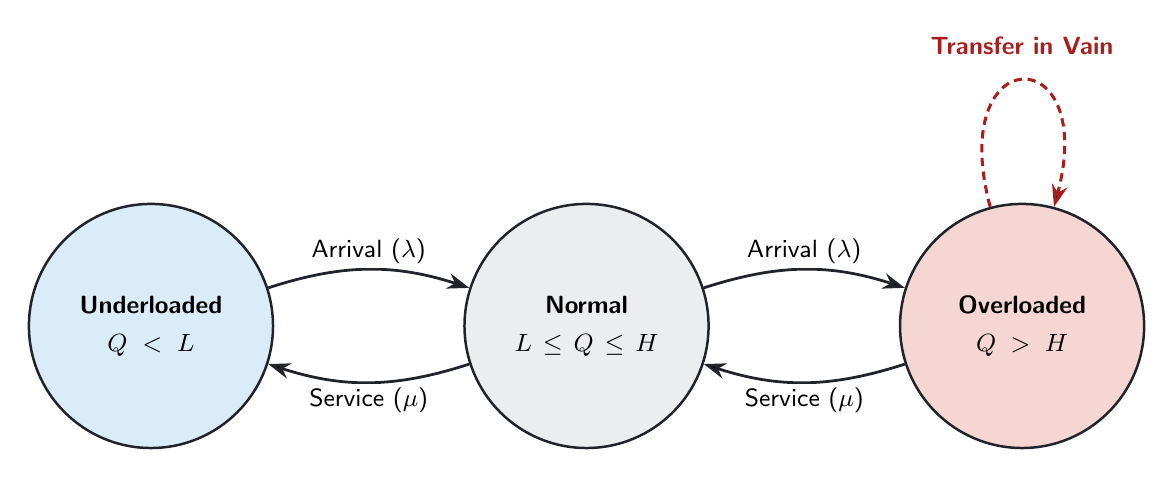
\begin{tikzpicture}[
    font=\sffamily,
    state/.style={
        circle,
        draw=AkramInk,
        line width=0.9pt,
        minimum size=31mm,
        text width=25mm,
        align=center,
        inner sep=1mm,
        font=\sffamily\small
    },
    transition/.style={
        -{Stealth[length=2.8mm,width=2.0mm]},
        line width=1.0pt,
        draw=AkramInk
    },
    feedback/.style={
        -{Stealth[length=2.8mm,width=2.0mm]},
        line width=1.1pt,
        densely dashed,
        draw=AkramRed
    },
    edge label/.style={
        fill=white,
        inner sep=1.5pt,
        font=\sffamily\small
    },
    node distance=24mm
]
    \node[state, fill=AkramBlueFill] (underloaded)
        {\textbf{Underloaded}\\[1mm]$Q<L$};
    \node[state, fill=AkramGrayFill, right=of underloaded] (normal)
        {\textbf{Normal}\\[1mm]$L\leq Q\leq H$};
    \node[state, fill=AkramRedFill, right=of normal] (overloaded)
        {\textbf{Overloaded}\\[1mm]$Q>H$};

    \path[transition]
        (underloaded) edge[bend left=18]
            node[edge label, above] {Arrival ($\lambda$)} (normal)
        (normal) edge[bend left=18]
            node[edge label, above] {Arrival ($\lambda$)} (overloaded);

    \path[transition]
        (normal) edge[bend left=18]
            node[edge label, below] {Service ($\mu$)} (underloaded)
        (overloaded) edge[bend left=18]
            node[edge label, below] {Service ($\mu$)} (normal);

    \path[feedback]
        (overloaded) edge[loop above, min distance=17mm, looseness=7]
            node[above=2mm, font=\sffamily\small\bfseries, text=AkramRed]
            {Transfer in Vain} (overloaded);
\end{tikzpicture}

% Page 2: monotone CDF profiles for three traffic intensities.
% The exponential profiles reproduce the qualitative ordering reported in the
% paper; they are not a digitisation of unavailable numerical samples.
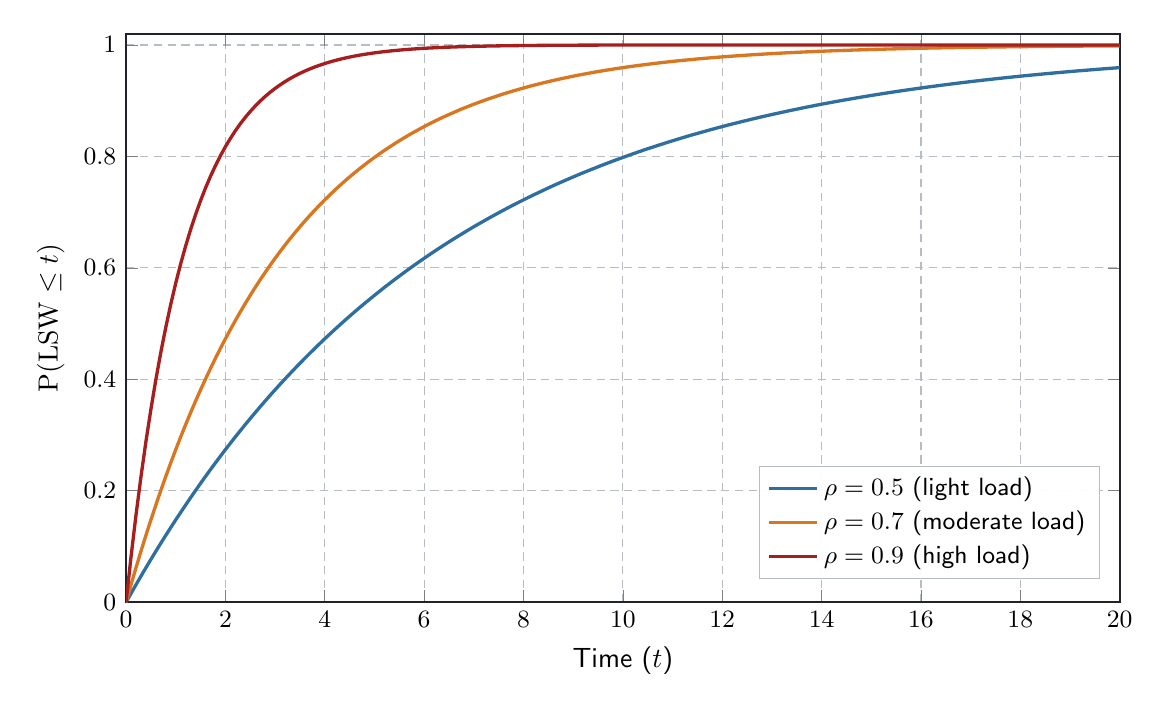
\begin{tikzpicture}[font=\sffamily]
    \begin{axis}[
        width=14.2cm,
        height=8.8cm,
        xmin=0,
        xmax=20,
        ymin=0,
        ymax=1.02,
        xlabel={Time ($t$)},
        ylabel={$\mathrm{P}(\mathrm{LSW}\leq t)$},
        axis line style={draw=AkramInk, line width=0.8pt},
        tick label style={font=\sffamily\small},
        label style={font=\sffamily},
        xtick={0,2,4,6,8,10,12,14,16,18,20},
        ytick={0,0.2,0.4,0.6,0.8,1.0},
        grid=both,
        major grid style={draw=AkramGrid, densely dashed, line width=0.45pt},
        minor grid style={draw=AkramGrid!60, dotted, line width=0.35pt},
        legend style={
            at={(0.98,0.04)},
            anchor=south east,
            draw=AkramGrid,
            fill=white,
            fill opacity=0.94,
            text opacity=1,
            font=\sffamily\small,
            cells={anchor=west}
        },
        domain=0:20,
        samples=201,
        no markers
    ]
        % Lower load: longer and more dispersed LSW duration.
        \addplot[AkramBlue, very thick] {1-exp(-0.16*x)};
        \addlegendentry{$\rho=0.5$ (light load)}

        % Moderate load: intermediate closure rate.
        \addplot[AkramOrange, very thick] {1-exp(-0.32*x)};
        \addlegendentry{$\rho=0.7$ (moderate load)}

        % High load: rapid, near-immediate LSW closure.
        \addplot[AkramRed, very thick] {1-exp(-0.85*x)};
        \addlegendentry{$\rho=0.9$ (high load)}
    \end{axis}
\end{tikzpicture}

\end{document}
